% Gemini theme
% https://github.com/anishathalye/gemini

\documentclass[final]{beamer}

% ====================
% Packages
% ====================

\usepackage[T1]{fontenc}
\usepackage{lmodern}
\usepackage[size=custom,width=106.68,height=60.96,scale=0.85]{beamerposter}
\usetheme{custom}
\usecolortheme{tntech}
\usepackage{graphicx}
\usepackage{booktabs}
\usepackage{tikz}
\usepackage{pgfplots}
\usepackage{pgf}
\usepackage{multicol}
\usepackage{mathtools}

% ====================
% Lengths
% ====================

% If you have N columns, choose \sepwidth and \colwidth such that
% (N+1)*\sepwidth + N*\colwidth = \paperwidth
\newlength{\sepwidth}
\newlength{\colwidth}
\setlength{\sepwidth}{0.02\paperwidth}
\setlength{\colwidth}{0.225\paperwidth}

\newcommand{\separatorcolumn}{\begin{column}{\sepwidth}\end{column}}

\newcommand{\minus}{\scalebox{0.75}[1.0]{$-$}}
\newcommand{\smallequals}{\scalebox{0.75}[1.0]{$=$}}
\newcommand{\sectionHeading}[1]{\vskip2.0ex \textbf{#1} \vskip0.25ex}

% ====================
% Title
% ====================

\logotitle{
\includegraphics[height=5.0cm]{Images/tntechgold.png}}
\title{Remote Controlled Tennis Ball Collector}
\author{Carter Brady \and Gabriel Dubose \and Cindy Escobar \and Tate Finley \and Ashli Watkins \and Maxwell Wynne }
\institute[shortinst]{Tennessee Technological University}
\qrcode{
\includegraphics[height=5.0cm]{Images/qrcode.png}}

% ====================
% Body
% ====================
\pgfplotsset{compat=1.16}
\begin{document}

\begin{frame}[t]
\begin{columns}[t]
\separatorcolumn

\begin{column}{\colwidth}

  \begin{block}{Project Overview}

    \sectionHeading{Description}

    \qquad Our capstone team reached out to the Tennessee Tech Tennis team. The Tennis team informed us that their current tennis ball mower was outdated and broken. This current model is operated by manually pushing the machine. This motion requires heavy exertion on the handlebar to make the machine move quickly. This sometimes causes the tennis balls to jam inside the machine from not pushing hard enough. The capstone team offered to solve the jamming problem along with adding remote control capability and an accurate ball counter to the collector for ease of use.
    
    \sectionHeading{Objective}

    \qquad The objective of this capstone project is to modify the existing tennis ball collector to have remote control capability, an accurate ball counter, and a vibration mechanism offering a modern solution to the Tennessee Tech Tennis team's tennis ball collector. 
    
    \sectionHeading{Specifications}
    
    \begin{itemize}
      \item The tennis ball collector shall be operated with a controller.
      \item The system shall collect and sense up to 100 balls at one time.
      \item The system shall indicate the number of tennis balls collected on a display.
      \item The system shall include a vibration mechanism to prevent tennis balls from jamming upon collection.
      \item For the safety of the system and the safety of others, the system shall be constructed using materials compliant with the U.S. Hazardous Materials Regulations. 

    \end{itemize}

  \end{block} 
    
    \begin{figure}
    \centering
    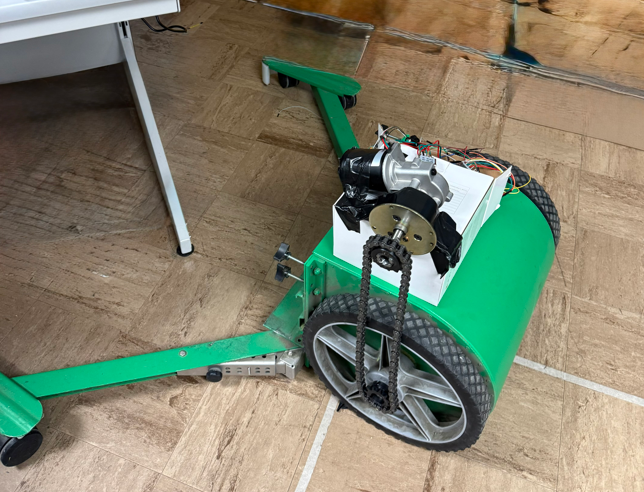
\includegraphics[width=20.0cm]{Images/RC_Collector_prototype.png}
    \caption{Modified tennis ball collector prototype.}
    \end{figure}
        
    \vskip3ex

\end{column}

\separatorcolumn

\begin{column}{\colwidth}
  \begin{block}{Block Diagram}
      \begin{figure}
        \centering
        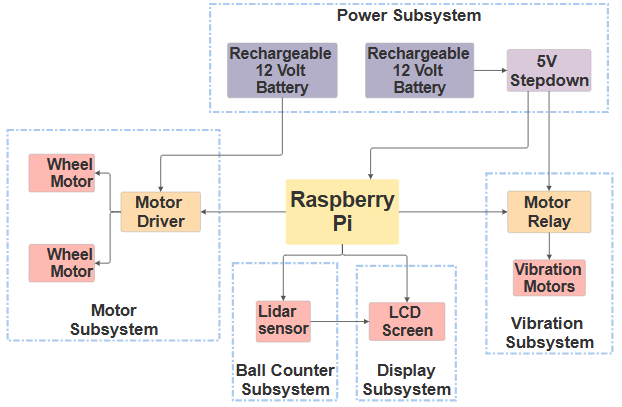
\includegraphics[width=22.0cm]{Images/Block_Diagram.png}
        \caption{Block diagram of tennis ball collector prototype and subsystems.}
      \end{figure}
  \end{block}
    
  \begin{block}{Project Subsystems}

    \vskip1ex
    \qquad \textbf{Power -} All electrical components of the system need to be supplied by a source. The goal of this system is to supply all the necessary power to the other components of the modified tennis ball collector.

    \vskip1ex
    \qquad \textbf{Remote Control -} To make the tennis ball collector remote controlled, the tennis ball collector's controls have to be coded and loaded onto the onboard miniature computer. The goal of this system is to code the required functionality of the collector's motions and onboard systems including the display.

    \vskip1ex
    \qquad \textbf{Counting Display -} The display subsystem keeps count on how many tennis balls are collected. Functionality like resetting the count number is done on a designated button of the controller.

    \vskip1ex
    \qquad \textbf{Counting Sensor -} Before incrementing the count on the display, a tennis ball has to be detected. The goal for this subsystem is to use a sensor to detect the tennis balls coming out of the collector and into the basket. This is done using light detection and ranging (LiDAR).

    \vskip1ex
    \qquad \textbf{Motor -} A tennis ball mower's collection mechanism is useless without the means to move the collector. The motor subsystem was built to be able to move the tennis ball collector at a consistent speed using controller inputs.

    \vskip1ex
    \qquad \textbf{Vibration -} To fix the jamming problem of the ball mower, a vibration system is integrated inside to help the tennis balls get unstuck. Then the tennis balls are able to be recollected more easily without getting stuck in the machine.

  \end{block}


\end{column}

\separatorcolumn

\begin{column}{\colwidth}


  \begin{block}{System Analysis}

    \sectionHeading{Experimental Tests}

    \begin{itemize} 
      \item \textbf{Sensing Accuracy Test -} Two LiDAR sensors were placed across from each other. The distance between them would be the same distance when mounted onto the collector. Then 10 tennis balls were rolled past the sensors for each trial at different speeds and angles. The counter on the display was recorded after each trial.
      \item \textbf{Controller Input Test -} The controller inputs were simulated using a python software script that recorded the button presses. A trial was conducted for each button used to control the collector's functionality. Each trial involved 5 button presses which tested the responsiveness of the buttons.
      \item \textbf{Battery Longevity Test -} A 12-Volt battery was fully charged then connected to the onboard motors. A stopwatch would track the amount of time the battery was still supplying power to the motors. The stopwatch was stopped when no power was being supplied to the motors.
    \end{itemize}

    \sectionHeading{Experimental Results}

    \begin{itemize} 
      \item \textbf{Sensing Accuracy Test - Success!} After 5 trials, the balls were counted correctly without any misses or double counts regardless of the speed and angle at which each ball was rolled across. 
      \item \textbf{Controller Input Test - Success!} Testing the seven inputs of the controller, each button showed perfect responsiveness and accuracy in button detection.
      \item \textbf{Battery Longevity Test - Underwhelming.} The battery ran for 1 hour, 20 minutes before the motor speed began to slow significantly, however, after 2 hours the battery lost the ability to recharge. 
      
    \end{itemize}

    \begin{figure}
    \centering
    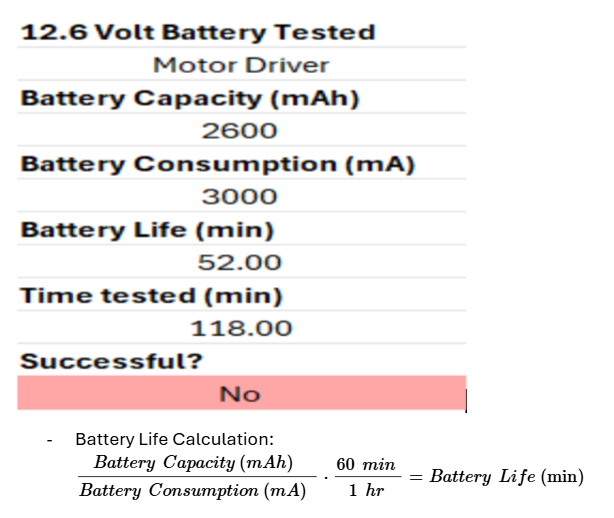
\includegraphics[width=20.0cm]{Images/battery_test_results.png}
    \caption{Battery Longevity Test results.}
    \end{figure}

  \end{block}

\end{column}

\separatorcolumn

\begin{column}{\colwidth}
  \begin{figure}
    \centering
    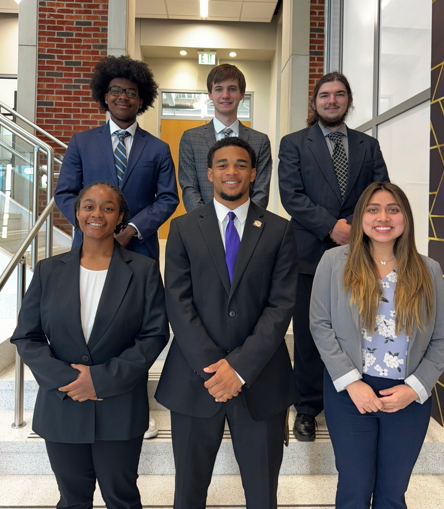
\includegraphics[width=19.0cm]{Images/Capstone_photo.png}
  \end{figure}
 
  \begin{block}{Conclusion}

    \qquad The total cost of the project was \$831.75 excluding the collector which was given to the capstone team by the customer. More prep work could be done in designing a printed circuit board specifically tailored to this project for better performance of the system. All constraints outlined were met except for the vibration subsystem which needed more testing and thought of practical implementation.

    \begin{table}
    \centering
    \resizebox{0.5\textwidth}{!}{
    \begin{tabular}{|c|c|}
        \hline
        Subsystem & Cost \\ \hline
        Power  & \$30.37  \\ \hline
        Remote Control  & \$84.99  \\ \hline
        Counting Display & \$13.57 \\ \hline
        Counting Sensor  & \$92.48  \\ \hline
        Motor  & \$449.94  \\ \hline
        Vibration  & \$17.37  \\ \hline
        Other Components & \$143.03 \\ \hline
        Total  & \$831.75  \\ \hline
    \end{tabular}
    }
    \caption{Bill of Materials.}
    \end{table}

  \end{block}
  
  \begin{block}{Acknowledgments}

    \vskip1ex
     \qquad This capstone team would like to acknowledge our instructor, Mr. Micah Rentschler; our advisor, Dr. Stephen Canfield; and our customer, Mr. Kenneth Doyle and the Tennessee Tech Tennis Team.   

  \end{block}
\end{column}
\separatorcolumn

\end{columns}
\end{frame}

\end{document}
